%%%%%%% SECTION %%%%%%%
\section{Architecture de communication hybride}

%\subsection{Introduction}

Dans la section précédente, l'introduction du modèle orienté événements 
s'intéresse principalement à ce qui se passe au sein d'un seul client. 
Or la collaboration passe par la mise en relation des différents collaborateurs, mais aussi par  
l'échange des données nécessaires à la collaboration (données de connexion, 
mises à jour de la scène, sensibilisation\dots)
Afin de pouvoir proposer un \gls{SEC} adapté aux besoins de l'édition de scènes 
3D, plusieurs types de granularité sont à distinguer : 
\begin{itemize}
	\item une granularité fine pour l'édition massive ;
	\item une granularité liée aux spécificités de la modélisation \gls{3D} ;
	\item et une granularité reposant sur des technologies web (réseau, interface, 
	interaction \gls{3D}).
\end{itemize}

Les systèmes \gls{P2P} qui sont orientés événements consistent en plusieurs 
n\oe uds interconnectés dont les fonctions et l'exécution des tâches sont
similaires. Les pairs partagent directement leurs ressources (contenu, CPU, 
stockage, bande passante) sans nécessiter de serveur central. A la place, les 
pairs coopèrent au moyen d'événements qui prennent la forme de messages lorsqu'ils
se les échangent. Les systèmes \gls{P2P} sont capables de s'adapter aux 
dysfonctionnements et à la dynamicité des pairs, tout en maintenant des 
performances acceptables. Les systèmes \gls{P2P} sont généralement utilisés 
comme soutien aux services de l'application pour la communication et la 
collaboration, le calcul distribué, la distribution de contenus et pour les services 
d'intergiciel comme le routage et la localisation, ou encore l'anonymat et la confidentialité.

\paragraph{Constat} Les \glspl{SEC} ont connu un fort développement avec 
l'intérêt 
croissant 
pour le \gls{P2P} dans les années 2000. 
La base théorique des \glspl{SEC} s'appuie sur les propriétés de 
convergence, préservation de la causalité et préservation de l'intention du modèle 
\acrshort{CCI} \cite{Sun1998}. 
La plupart des travaux liés aux \glspl{SEC} \gls{P2P} s'intéressent à 
l'édition collaborative massive de documents textuels dont les propriétés 
de commutativité sont plus faciles à gérer (insertion / suppression) en 
comparaison à celles concernant la \gls{3D} (multiplication de matrices de 
rotation). La génération de conflits en \gls{3D} peut vite devenir incontrôlable. Il est 
donc nécessaire de mettre en place des mécanismes de détection de 
conflits et de maintenir une cohérence au cours des sessions de 
collaboration. 





%\gls{WebRTC} est une technologie qui fournit aux navigateurs 
%\textit{destkop} et mobiles la possibilité de communiquer en temps-réel 
%(cf \ref{sec:webrtc} via une collection de standards, 
%protocoles et \glspl{API} JavaScript. 
%L'un des atouts de cette technologie est de permettre de façon simple et 
%sans module d'extension la capture d'un flux audio et / ou vidéo (ex : 
%applications de VoIP), ainsi que l'échange de données arbitraires entre 
%navigateurs sans nécessiter d'intermédiaires (ex : partage de fichiers en 
%\gls{P2P}).
%Techniquement, \gls{WebRTC} supporte un canal temps-réel 
%bidirectionnel pour l'échange de données. Contrairement à 
%\gls{WebSocket}, qui est basé sur \gls{TCP}, \gls{WebRTC} repose sur 
%\acrshort{UDP} en intégrant une pile de plusieurs protocoles (Figure 
%\ref{fig:protocolstack}) qui lui offre des fonctionnalités similaires (fiabilité, 
%ordonnancement, sécurité). 

%TODO parler chargeet distribution


\paragraph{Contribution}
La mise en place d'une architecture de communication 
hybride permet de concilier à la 
fois les avantages d'une architecture client-serveur et ceux du \gls{P2P}, en évitant 
certains désavantages occasionnés dans ces derniers (engorgement du serveur, 
pair seul sur le réseau\dots). 
Le terme \og hybride\fg{} invoque un compromis entre la 
centralisation de l'information nécessaire à la prise de décision globale et 
la décentralisation des échanges utile à l'amélioration du partage de 
contenus \gls{3D} à l'échelle locale. 
En agissant sur ces deux échelles, la granularité de la collaboration est plus fine. 
Par exemple, le passage à l'échelle est facilité par la présence de 
ressources locales et la coordination des utilisateurs se fait à une échelle 
globale, ce qui permet également l'accès à une source de vérité 
centralisée (base de données) et commune.
Dans le contexte des \glspl{EVC3D}, le but 
est d'obtenir une architecture de communication : 

\begin{itemize}
	\item entièrement basée web ; 
	\item robuste face à l'évolution du nombre de collaborateurs ; 
	\item efficace en termes d'accès et de distribution de la donnée ; 
	\item et qui s'adapte à l'échelle selon les besoins de la collaboration.
\end{itemize}


Tous les travaux liés à cette thèse 
\cite{Desprat2015a,Desprat2015b,Desprat2016,Desprat2017} s'appuient sur une 
architecture de communication hybride tripartite (Figure \ref{fig:hybrid}) pour 
faire de la modélisation \gls{3D} collaborative : serveur, persistance 
et les pairs\footnote{Les pairs sont appelés \og Clients\fg{} dans les premiers 
travaux}. 

Les contributions portées par Desprat et al. dans \cite{Desprat2015a} et \cite{Desprat2015b} 
s'appuient sur des pairs ayant un rôle simple et proposent une transmission des 
mises à jour en tant que différentiel d'état. Les conflits lors d'opérations 
concurrentes sont évités grâce à un mécanisme de verrouillage. 
Plus tard, dans \cite{Desprat2016}, les auteurs mettent en place le modèle 
orienté événements qui impose l'évolution, au niveau réseau, du protocole 
de transmission (celui-ci reposant sur 
des notifications d'événements et la gestion des flux d'agrégat). 
Plus récemment, dans \cite{Desprat2017}, est apparue la distinction entre 
les deux rôles parmi les pairs : la 
partie serveur se compose désormais de pairs qui ont un rôle de vérification 
de la cohérence et de relais des données dans la couche \gls{P2P}. Cette 
contribution intervient dans le but d'encourager la résilience du système et la 
vitesse de dissémination des informations dans le réseau, en favorisant la prompte 
détection de conflits (source de vérité plus proche des pairs producteurs). 
Cette extension repose sur la présence d'un journal d'événements partagé et 
répliqué sur les pairs participants à la collaboration.

\begin{figure}[h!]
	\centering
	\includegraphics[width=0.7\columnwidth]{eps/hybrid5.eps}
	\caption{Architecture hybride tripartite : serveur, persistance 
		et les pairs.}
	\label{fig:hybrid}
\end{figure}

Cette section décrit le modèle d'architecture mis en 
place pour gérer la transmission de contenu entre les différents clients 
qui participent à l'édition collaborative d'un espace de travail \gls{3D} partagé. 
Les différents protocoles de transmission, issus des travaux sus-nommés, 
sont présentés. Ils montrent ainsi l'évolution de l'architecture de communication de 
sa version naïve à la version étendue, plus proche des considérations métiers et 
offrant plus de liberté dans la création grâce la mise en place d'un système inspiré 
des \glspl{CRDT}.
 
Les différents éléments constitutifs d'un pair sont détaillés avant la présentation 
des deux types de pairs rencontrés dans l'architecture.
Sont expliqués ensuite les mécanismes de mise en relation de 
ces composants pour que les différents participants d'une session 
collaborative puissent communiquer de manière transparente, cohérente et 
résiliente.

%TODO reprendre pour partie implantation
%Les travaux présentés s'inscrivent dans un contexte où les besoins 
%d'interopérabilité et de standardisation sont élevés pour permettre à des 
%utilisateurs de prendre le système rapidement en main sans installer autre chose 
%qu'un navigateur. 


\subsection{Éléments constitutifs d'un pair}
Dans un réseau \gls{P2P}, chaque pair est considéré comme un système à part 
entière qui contient ses propres problématiques d'implémentation. Avant de 
présenter la contribution liée à l'intergiciel dans 3DEvent, il est nécessaire 
d'introduire les composants et les fonctions clés qui constituent un pair du point de 
vue strictement réseau en 
présentant une vue minimaliste d'un pair dédié au partage de contenu 
\cite[p.135-136]{Buford2009}. Les 
fonctions sont divisées en trois :
\begin{itemize}
	\item la couche de routage et d'échange de messages ;
	\item la recherche et le stockage de contenu ;
	\item ainsi que la configuration et sélection du rôle du pair.
\end{itemize}


\begin{figure}[ht]
	\centering
	\inputTikZ{0.8}{eps/tikz/middleware/middleware}
	\caption{Composants de chaque pair dans 3DEvent (point de vue réseau)}
	\label{fig:middleware}
\end{figure}


Chaque pair générique fournit de base une \gls{API} pour les fonctions d'échange 
de messages et de recherche. 
L'\gls{API} de recherche est principalement en lien avec le 
gestionnaire d'instances qui se charge de la recherche, mais il est possible de se 
connecter à des pairs via d'autres pairs si le serveur est absent ou pour renforcer 
le maillage.
L'élément responsable de la couche de routage et d'échange de messages permet 
à chaque pair de maintenir un état de connexion avec ses voisins dans la couche 
; maintenir cet état inclut la découverte de voisins et la maintenance  à jour des 
états des voisins.
Un pair possède un mécanisme d'amorçage (\textit{bootstrap}) qui permet de 
localiser les autres pairs qui lui permettront de rejoindre la couche \gls{P2P}. Les 
étapes pour rejoindre ou quitter la couche sont proposées par le protocole 
d'établissement de connexion 
(cf signaling mecanism\todo{ref section signaling}).
La couche applicative permet  d'échanger des messages avec les autres pairs 
dans le réseau en utilisant l'\gls{API} réseau, et les messages reçus peuvent être 
transférés à leur destination en utilisant la fonction de transfert de messages. 

Le contenu partagé est stocké localement pour pouvoir être accessible par d'autres 
pairs, ainsi que l'interface de l'application du pair courant. Le contenu doit être 
organisé pour la recherche d'informations afin de fournir une indexation et une 
interface de requête. 
L'espace de stockage pour les données partagées va correspondre aux différents 
états des agrégats \cite{Desprat2015a,Desprat2015b} ou au journal d'événements 
\cite{Desprat2016,Desprat2017}.


La dernière fonction concerne la manière dont le pair auto-organise, à la fois, ses 
ressources locales et son rôle dans le réseau. Le pair détermine les 
ressources du système et du réseau disponibles et peut surveiller les 
changements éventuels régulièrement.
Le pair a connaissance du rôle qui lui est attribué à sa création dans le réseau. Les 
rôles des pairs (super pair, relai, producteur\dots) dépendent de 
capacités comme les ressources du système et du réseau. Le rôle induit les 
capacités et la configuration de chaque pair, i.e. un pair actif est configuré 
uniquement pour produire, stocker et relayer les données tandis qu'un pair passif ne fait que stocker et relayer les données. La stabilité du pair peut être indiquée par son niveau de 
\textit{churn} (dynamicité : rejoindre et quitter un réseau) par exemple. 
La Figure \ref{fig:middleware} peut être affinée en fonction du type de 
réseaux et d'applications. Chaque pair comprend un protocole pour la gestion
de sessions (ex: REST API) et pour l'échange de données (ex: RTCDataChannels)  
pour pouvoir participer à la collaboration.



Les architectures de communication des contributions se divisent en deux parties, 
chacune correspondant au paradigme qu'elles utilisent respectivement : état ou 
événement. Selon le paradigme auquel elles font référence, elles peuvent 
être décrites par plusieurs critères:
\todo{revoir}
\begin{description}
	\item[Spécificité des composants de l'architecture] Les pairs sont la base de la 
	dissémination de l'information. La partie serveur 
	centralise les données liées à la persistance long  terme et
	décentralise la réplication des données à court terme. Cela évite au 
	serveur 
	d'être le point central des échanges en déchargeant les canaux passant par le 
	serveur.
	\item [Gestion de la session] 
	La gestion de la session suit le cycle de vie des pairs au sein du réseau 
	lorsqu'ils participent à une session collaborative. 
	Pour intégrer le réseau \gls{P2P} et participer à l'édition d'une scène \gls{3D} de 
	manière collaborative, les clients passent par les étapes suivantes :
		\begin{enumerate}
		\item Phase de \textit{signaling}
		\label{phase1signaling}
		\begin{enumerate}
			\item Signification de la présence auprès du serveur de \textit{signaling}
			\item Récupération de la liste des identifiants des pairs auxquels se 
			connecter
			\item Création d'une connexion \gls{P2P} avec les autres pairs
			\item Souscription aux flux
			
		\end{enumerate}
		\item Phase de synchronisation
		\label{phase2sync}
		\begin{enumerate}
			\item Requête des données manquantes
			\item Récupération des données manquantes
			\item Ré-ordonnancement des messages reçus
			\item Maintien de la cohérence (détection de conflit)
		\end{enumerate}
		
		\item Phase de génération de nouvelles données valides 
		\label{phase3gen}
		\begin{enumerate}
			\item Publication des données aux voisins
		\end{enumerate}
		
		\item Phase d'abandon
		\label{phase4quit}
		\begin{enumerate}
			\item Notification aux voisins 
			\item Fermeture des canaux
		\end{enumerate}
	\end{enumerate}
	
	Ces quatre phases sont distinctes même si, lorsqu'un pair initialise ou rejoint 
	une 
	session collaborative (séquence d'initialisation), les phases 
	\ref{phase1signaling}, \ref{phase2sync} et \ref{phase3gen} s'enchainent pour 
	ce pair. Durant la session collaborative, les phases \ref{phase2sync} et 
	\ref{phase3gen} s'alternent. La phase \ref{phase4quit} se produit lorsque qu'un 
	client quitte une scène de manière volontaire (changement de scène, fermeture 
	de l'onglet du navigateur) ou involontaire (fausse manipulation, navigateur en 
	panne, coupure internet) signifiant la fin de la session collaborative.
	
	\item [Gestion du stockage et structure des données] 
	Le stockage peut prendre plusieurs formes : \textit{in-memory}, stockage local, 
	disque dur\dots selon le type de stockage adapté et disponible. 
	Dans l'architecture hybride, il existe deux niveaux de stockage : la persistence 
	long-terme, distante -- la base de données -- et la persistence court-terme, 
	locale -- le navigateur.
	Le serveur assure, d'une part, la centralisation du stockage à long-terme, et 
	d'autre part, la mise en relation des différents clients.
	\item [Gestion de la synchronisation et de la cohérence (détection des conflits)] 
	Il existe différentes possibilités de synchronisation des pairs. 
	
	L'édition concurrente lors de la collaboration peut être gérée de différentes 
	manières, selon si elle est plutôt pessimiste ou optimiste lors de la réplication 
	des 
	données (voir Section \ref{sec:concurrence}). L'intégration d'une solution ou 
	l'autre 
	a de lourds impacts sur l'expérience utilisateur (fonctionnalités, interface 
	utilisateur) et la gestion de la cohérence dans le réseau \gls{P2P}.  
	
	\item [Protocole d'échange]
	La couche \gls{P2P} fournit une dissémination rapide de l'information et 
	\todo{finir}
\end{description}


%
%\subsection{Architecture de communication \og orientée états\fg{}}
%\label{sec:comm_state}

\subsection{Architecture hybride \og orientée états\fg{}}
\label{sec:comm_state}

Les premiers travaux liés à cette thèse \cite{Desprat2015a,Desprat2015b} se sont 
intéressés principalement à la mise en place de l'architecture de communication 
en basant les structures de données sur des états (plutôt que des événements). 
Cette section décrit les choix faits lors de la modélisation de l'architecture \og 
orientée état\fg{}, pour le stockage et le transfert par exemple, en lien fort avec les 
technologies web sous-jacentes. 

%  well for web distributed sys- tems even if mobile devices should have limited 
%  perfor- mance due to back and forth requests that are energy consuming.
%  
\subsubsection{Spécificité des composants de l'architecture}
Le système présenté repose sur une architecture \acrshort{REST} 
(\acrlong{REST}) concernant les échanges clients-serveur. Cette architecture 
permet de séparer les responsabilités entre le client et le serveur en séparant 
l'\gls{IU} du stockage. \gls{REST} propose une interface uniforme. Cela implique 
que chaque ressource est identifiée et manipulable par des représentations définies 
(modification, suppression). 

Chaque pair correspond a un client (navigateur web) qui contient l'intergiciel 
\gls{P2P} offrant des fonctionnalités limitées, l'interface utilisateur contenant 
l'environnement \gls{3D} et un espace de stockage reposant local (IndexedDB).

La persistance long terme est une base de données NoSQL. Ce type de bases de 
données a tendance à être optimisée en lecture (grâce à un 
langage de requête dédié) et permet d'éviter les 
structures rigides. Cette flexibilité est utile lors du stockage des modèles \gls{3D} 
et 
encourage la conservation d'autres métadonnées (ex: relations entre les différents 
objets) pour faciliter la traçabilité. 
Avec une base de données centralisée, le système possède une source de 
données fiable et autoritaire qui permet à un utilisateur de récupérer le bon contenu 
quand il revient sur une scène. La totalité du document, contenant la scène, est 
envoyé à l'utilisateur lorsqu'il y accède.


\subsubsection{Gestion du stockage et structure de données}

Avec une base de données NoSQL utilisant des schémas dynamiques, les 
données sont stockées sous forme de document. Chaque document est 
auto-descriptif et peut contenir des valeurs qui s'imbriquent sous la forme d'une 
structure en arbre hiérarchique. Une collection consiste à grouper des documents, 
équivalent, dans une base de données relationnelle, à la notion de table. La base de 
données contient deux types de collections : les scènes et les géométries. Une 
collection de scènes contient des scènes qui sont décrites par leur identifiant et 
les méta-données de l'espace virtuel \gls{3D}, ainsi que la liste des contributeurs et 
la 
liste des maillages. Cette liste correspond à une association entre un identifiant de 
maillage, les méta-données de l'objet et l'identifiant d'une géométrie existante. 
Les géométries sont, quant à elles, stockées avec leur identifiant propre et l'objet 
3D complet donné sous le format \gls{JSON}.

Sur chaque pair, il existe un stockage relationnel pour 
chaque objet de la base de donnée récupérée. Cela permet au client de faire des 
requêtes directement dans son espace local si besoin, par exemple en ajoutant un maillage. 
C'est également une source pour transférer ses modifications aux autres clients.
Les navigateurs permettent désormais de stocker des quantités de données 
importantes localement avec une durée de vie illimitée. 
Les paramètres des opérations fondamentales effectuées sur la base de données 
(\gls{CRUD}) sur les collections sont très bien supportés par les requêtes 
\gls{REST}.



%
%We propose to auto connect users on a scene with a We- bRTC connection. As 
%each user send their ID to the database at their arrival, they also retrieve those 
%which where already present on the scene. We are able to cre- ate a full mesh 
%topology network in order to make them communicate the updates.
%
%Even if we have a full mesh topology, the P2P message layer is more similar 
%the 
%star topology. Indeed, the Fig- ure 2 shows the path of a sent message 
%operation 
%on the connection and it is only sent to the one degree neigh- bors of the original 
%broadcaster (the “B” node on the Figure 2).
%
%
%We choose to keep reliable and in order delivery for now. The RTCDataChannel 
%API supports many data types (strings, binary types: Blob, ArrayBuffer. . . ). 
%These types are helpful in a 3D multi user environment to broadcast messages 
%including the objets and their transformations. We tried to limit the amount of 
%data 
%by sending only relevant information but there is actually no particular 
%optimization. The channel can be over- feed when an object is imported then 
%pushed through the network.
%

\subsubsection{Gestion de la synchronisation et de la cohérence}
\label{sec:synchronisation-client-serveur}

Les travaux \cite{Desprat2015a} et \cite{Desprat2015b} présentent une version 
naïve du processus de synchronisation. La cohérence est garantie par un système 
de verrouillage des objets. Cela évite notamment les sélections concurrentes et par 
conséquent les éditions concurrentes. 
Lors de la récupération de la scène, elle est considérée comme cohérente. 
Ensuite, le choix d'avoir des connexions \gls{P2P} ordonnées et fiables, ainsi 
qu'un maillage de pair complet, implique que toute donnée envoyée par un pair est 
forcément reçue par les autres. 
L'échange des mises à jour entre le client (persistance à court terme) et la 
base de données (à long terme) leur permet de se synchroniser dans un premier 
temps. La base de données peut également servir en cas de conflits importants ; 
elle sert de référence.

Lors de la connexion d'un nouveau client, a lieu la synchronisation des deux 
systèmes de persistance pour obtenir les mises à jour : 

\begin{enumerate}
	\item depuis le client, où l'on distingue trois cas :
	\begin{enumerate}
		\item travail "\textit{offline}" (hors ligne) : l'utilisateur a travaillé hors ligne et 
		doit maintenant publier "en ligne" son travail. Les mises à jour sont publiées 
		sur la base de données ; le serveur vérifie si aucun conflit ne survient puis 
		fusionne (\textit{merge}) les nouvelles entrées avec l'existant; 
		
		\item travail "\textit{serverless}" (en collaboration avec entre pairs sans le 
		serveur) : dans le cas où le serveur est absent, les clients peuvent continuer 
		de créer en collaborant. Ces données n'étant stockées que sur le client, il est 
		nécessaire de les transmettre à la base de données dès qu'une connexion 
		est possible. 
		
		\item travail "\textit{online}" (en collaboration entre pairs comprenant la partie
		serveur) : le client systématiquement ses 
		nouvelles modifications pour qu'elles soient intégrées à la base de données.
	\end{enumerate}
	\item depuis la base de données :
	Le client reçoit toutes les nouvelles mises à jour de la scène depuis la dernière 
	fois qu'il s'est connecté. Cela peut également inclure des mises à jour qui sont 
	en conflit avec ce qu'il y a dans son propre espace de stockage, qu'il lui faut 
	donc modifier.
	Dans le cas où un seul utilisateur est connecté, la base de données est la 
	seule source disponible pour la mise à jour du client. 
\end{enumerate}


Le fait de synchroniser un client avec une base de données NoSQL dès que cela 
est possible permet de supporter les connexions intermittentes comme pour les 
appareils mobiles dans cette architecture ; cette approche est connue sous le nom 
de \og\textit{offline first}\fg{} \cite{Gadea2016}.
\subsubsection{Topologie et protocole d'échange}
Cette architecture est basée sur une topologie de maillage complet (\textit{full 
mesh topology}) pour le réseau \gls{P2P}.
Les échanges se font donc à deux niveaux: entre les pairs, ainsi qu'entre chaque 
pair et la base de données. Pour le premier niveau, la couche réseau \gls{P2P} est 
assez 
naïve dans le sens où les connexions sont considérées comme fiables et 
ordonnées ; le client n'a alors qu'à publier toutes les modifications qu'il effectue et 
les envoyer à tous les clients (auxquels il est nécessairement connecté).
Les pairs échangent des différentiels d'état sur les objets. Ces messages ne 
contiennent pas d'information sémantique sur le type d'action effectuée par chaque 
utilisateur. 

\subsubsection{Discussion sur les architectures de 
communication orientée \og états\fg{}}

La base de données centralisée est beaucoup sollicitée lors des sessions 
collaboratives, ce qui peut mener à une surcharge similaire aux architectures 
uniquement client-serveur. 
En combinant client-serveur et \gls{P2P}, la charge aurait dû être réduite et 
transférée aux autres pairs, notamment lors de la phase de récupération d'une 
nouvelle scène qui repose entièrement sur le serveur. 
Chaque pair assume la responsabilité dans l'envoi de ses modifications à tous les 
autres pairs. Cette tâche ne profite pas du réseau \gls{P2P} de manière optimale 
car la topologie ne profite pas de la fonction relais des pairs. Cela pourrait alléger  
la distribution dans la couche \gls{P2P} et responsabiliser un peu plus les pairs 
pour faciliter le passage à l'échelle.
En effet, la topologie en maillage complet limite le passage à l'échelle car le 
nombre de connexions va croître de manière exponentielle. 

Par ailleurs, les requêtes \gls{CRUD} ne sont pas très expressives concernant le 
métier. 
Aucune vérification n'est donc effectuée sur la validité des données transmises 
dans cette architecture. De plus, il peut arriver, du fait de latences réseaux que les 
modifications des différents utilisateurs s'entrelacent à l'arrivée et ne rendent pas 
l'intention de l'utilisateur. Cela peut mener à des dé-synchronisations fortes.

Concernant la gestion de la concurrence, l'utilisation d'une solution pessimiste 
dans un environnement \gls{P2P} peut parfois mener à des inter-blocages si un 
utilisateur quitte la scène sans avoir relâché l'objet, c'est à dire sans en avoir 
informé la base de données et les autres 
utilisateurs. 
Même si l'application peut prendre le relais et permettre la relâche du 
verrou au bout d'un certain temps, l'expérience utilisateur peut être dégradée 
pendant cette période.
Le maintien de la cohérence est garanti dans ce modèle si l'on 
considère un environnement où la fréquence des modifications n'est pas très 
élevée, et que tous les clients communiquent leur horloge locale pour établir un 
référentiel de temps concernant les mises à jour. 

Enfin, le transfert par différentiel d'état utilisé pour réduire la taille des 
données liées au changement d'état des objets lors de la transmission des 
données peut varier grandement selon le type de changement 
effectué, rendant peu prévisible la charge des canaux de communication. 
%
%Some issues remain in RTCDataChannel API : the com- patibility and 
%interoperability is still not complete be- tween browsers6, some browsers (like 
%Chrome) im- pose a send limit (about 6MB) for the data transmitting through 
%DataConnections and the security of the com- munication is still vulnerable7. 
%The 
%system overview (Figure 4) illustrates the communication architecture topology 
%between the peer clients and server (plus sig- naling).



%\subsection{De l'état à l'événement}
%\label{sec:statetoevent}

\subsection{De l'état à l'événement}
\label{sec:statetoevent}
Afin d'intégrer la notion d'historique dans une application web, plusieurs indicateurs 
sont nécessaires (version, granularité de l'historisation, type et taille des données 
manipulées). Cette section décrit le processus pour passer d'un système basé 
états à un système basé évènements dans l'intérêt de réduire la somme des 
données transmises sans perdre d'information concernant la logique métier.
\paragraph{Description des variables}
Une scène $S$ contient l'ensemble des $n$ objets $x$ ($S =\{x_0,x_1,...,x_n\}$). 
Chaque élément de $S$ est associé à une taille calculée comme la somme des 
modifications $m$ selon la version $v$. 

Pour tout objet $x$ appartenant à la scène $S$ on associe une taille $w \in 
\mathbb{R}$. $w$ correspond à la taille totale des données transmises pour 
modifier l'objet à chaque version $v$ ($v$=0 correspond à la taille de l'objet à l'état 
original, i.e. l'\gls{EventStore} est vide). La taille totale de la scène, notée $Sw$, 
correspond à sommer la taille de tous ses objets (équation \ref{eq:sw}). Toutes les 
variables évoquées sont exprimées en octet pour avoir des termes avec des 
unités homogènes.

\begin{equation}
\label{eq:sw}
\text{Taille d'une scène $S$ : } S_w= \sum_{i=0}^{n}w_i
\end{equation}


\paragraph{Transmission par état}
Dans un système où à chaque modification on transmet l'état complet (équation 
\ref{eq:complet}), la taille des éléments transmis correspond à la somme de tous 
les états par lesquels l'objet est passé. Cette valeur va augmenter par paliers de 
tailles relativement équivalentes.
La transmission par état permet d'avoir un historique grâce à une sauvegarde 
chronologique. Cependant elle est lourde voire redondante et n'offre pas 
d'information sur l'intention de l'utilisateur (quelle opération a permis d'arriver à cet 
état?).

\begin{equation}
\label{eq:complet}
\text{Par état : } w_i = \sum_{v=0}^{n}state_{v}
\end{equation}


\paragraph{Transmission par différentiel d'état}
\label{par:diff}
Dans un système où l'on transmet un différentiel d'état (équation 
\ref{eq:différentiel}), la différence entre deux états peut être difficile à exprimer 
\info{cf meshhisto} car il s'agit d'un objet 3D dont les informations, stockées dans 
un fichier, ne sont pas linéaires. Le différentiel peut beaucoup varier jusqu'à 
atteindre une taille proche de l'état actuel si une transformation génère beaucoup 
de modifications par rapport à l'état précédent. A contrario, une modification sur la 
position d'un objet peut être très légère. La fonction représentant la taille des 
ressources transmises augmentera par palier avec au pire les propriétés de la 
proposition précédente (équation \ref{eq:complet}). Le différentiel d'état permet 
d'alléger la transmission par rapport à la proposition précédente, ne contenant 
cependant pas d'information sémantique sur ce qui est transmis et les opérations 
qui ont conduit à l'état d'un objet 3D de la scène.

\begin{equation}
\label{eq:différentiel}
\text{Par différentiel d'état : } w_i = state_0 + \sum_{v=1}^{n}(\underbrace{state_{v} 
- state_{v-1}}_{differential})
\end{equation}

\paragraph{Transmission par évènement}
La transmission par évènement (équation \ref{eq:evenement}) repose sur le 
principe du différentiel d'état ($differential$) exprimé ci-dessus (équation 
\ref{eq:différentiel}) en ajoutant la notion de type d'évènement ($eventType$). Le 
type d'un évènement indique le nom de la transformation à appliquer pour passer 
d'un état à l'autre. Un évènement contient par nature une sémantique <<métier>> 
associée à chaque opération qui donne des indications sur l'intention de 
l'utilisateur. 

\begin{equation}
\label{eq:evenement}
\text{Par évènement : } w_i= state_0 + \sum_{v=1}^{n}(\underbrace{eventType + 
differential}_{event}) 
\end{equation}

Dans un \gls{EVC3D}, il y a des évènements concernant à la fois la manipulation 
3D, la navigation et les éléments se rapportant à la collaboration (par exemple: 
prendre le point de vue d'un collaborateur). La taille d'un évènement est variable 
(comme un différentiel d'état) avec un minimum contenant le type d'évènement 
($eventType$) dû à sa structure type/paramètres. Cette proposition est un peu 
plus lourde à transmettre que la précédente mais ajoute une valeur sémantique à 
l'historique.



%\subsection{Architecture de communication \og orientée événements\fg{}}
%\label{sec:comm_event}

\subsection{Architecture de communication hybride \og orientée 
événements\fg{}}
\label{sec:comm_event}

Cette architecture est une combinaison des contributions présentées dans 
\cite{Desprat2016,Desprat2017} : elle repose sur les éléments du 
framework orienté événements (Section \todo{ref modele event}) qui sont également 
en relation avec la couche réseau (Figure \ref{fig:archievent}).
\begin{figure}[ht]
	\centering
	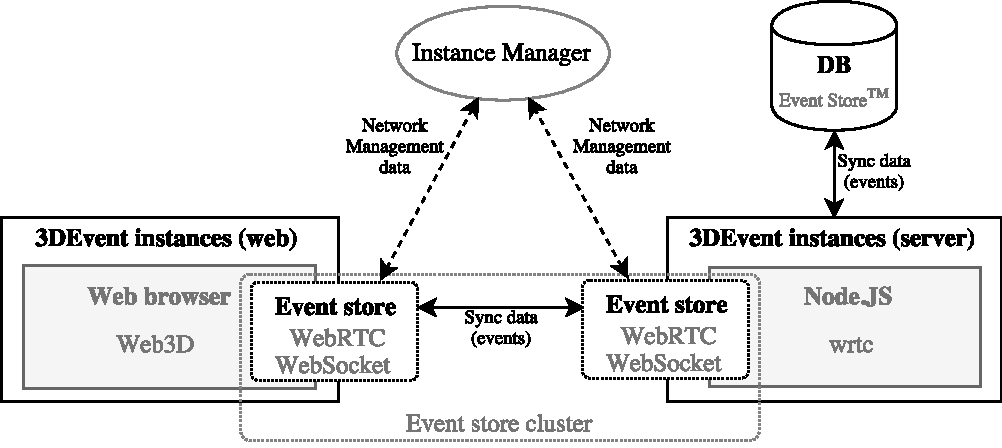
\includegraphics[width=\columnwidth]{eps/archi.pdf}
	\caption{Architecture de communication \og orientée événements\fg{}}
	\label{fig:archievent}
\end{figure}

\subsubsection{Spécificité des composants de l'architecture}
L'Event Store est un composant clé dans le traitement des événements. Présent 
sur chaque pair, il prend en entrée des événements de deux natures : ceux qu'il a 
générés via la partie commande (internes) et ceux reçus via le réseau 
principalement (externes). 
L'Event Store produit en sortie des événements dits \og 
cohérents\fg{} qui peuvent être publiés par la suite sur l'Event Publisher.
Un Event Store est composé de deux types d'éléments : 
\begin{itemize}
	\item l'\gls{ESM} qui gère les flux d'événements : structure de données 
	présente dans chaque Event Store qui doit permettre l'accès en lecture et en 
	écriture des agrégats qu'elle contient. 
	Un \gls{ESM} contient des flux d'événements ordonnés temporellement 
	pour chaque agrégat géré ;
	\item les \glspl{NB} qui servent de connecteurs réseaux : responsables de la 
	gestion d'une connexion \gls{P2P}, i.e. gère le flux de données entrant et 
	sortant vers chaque pair auquel ils sont reliés.
\end{itemize}

La Figure \ref{fig:archievent} montre des pairs (appelés instances) de différentes 
natures :
\begin{itemize}
	\item Instance Web :  produit, stocke et relaie des événements aux autres 
	instances.
	\item Instance Serveur : stocke et relaie des événements aux autres instances 
	et à la base de données. 
\end{itemize}

En plus de servir de relais comme une Instance Serveur, une Instance Web est 
productrice d'événements. C'est en général le type d'instance par lequel un 
utilisateur accédera à l'application. Les Instances Serveurs, en comparaison avec 
l'architecture présentée précédemment, sont des \og serveurs\fg{} qui participent 
directement à la couche réseau. En cela, ils aident à la dissémination des données 
et peuvent rapidement être montés pour garantir une disponibilité des données 
auprès des autres instances (notamment en cas de panne).
Toutes les instances sont coordonnées par l'\gls{IM} qui est responsable de mettre 
les pairs en relation. Il est notamment le serveur responsable dans le mécanisme 
de \textit{signalling}. 

L'ensemble des Event Stores forme une grappe (\textit{cluster}) qui gère le 
journal d'événements partagé de manière répartie entre toutes les instances.
\subsubsection{Gestion du stockage}
\paragraph{Local avec l'\gls{ESM}}
Lorsque l'Event Store reçoit de nouveaux événements, l'\gls{ESM} crée ou 
récupère le flux d'événements associé à l'agrégat dans un premier temps. Puis, il 
stocke l'événement à la suite de ceux présents dans le flux de l'agrégat.

\paragraph{Long-terme et distant avec une base de données fonctionnelle}
Dans un contexte industriel de collaboration, l'information doit être disponible sur le 
long-terme, facilement accessible par l'entreprise. La persistance à 
long-terme stocke le journal d'événements qui est la 
source de vérité de l'application. Elle peut également stocker des projections 
prédéfinies, calculées à la volée ou encore des \textit{snapshots} de l'application.

Sur la base du modèle orienté événements, les données à stocker sont les 
événements. Ils sont immuables et 
constituent des données purement fonctionnelles\todo{voir section \gls{ES} vs CS}.
L'utilisation d'une base de données fonctionnelle permet de se reposer sur 
l'immuabilité des événements.
L'argument souvent opposé à l'utilisation de telles bases est le coût de l'espace de 
stockage. Or le coût de la redondance et de la non localité du traitement des 
données, a chuté au cours de ces dernières années. 
Une base de données dont les données muent -- i.e où chaque donnée peut être 
modifiée à n'importe quel moment -- ne permet pas de conserver l'historique des 
modifications (ex : \textit{Active Record}). Dans une base de données dite 
fonctionnelle, les données stockées sont immuables -- i.e. elles ne peuventt être modifiée \textit{a posteriori} et fait seulement référence à 
d'autres données immuables. Une telle base de données est \og \textit{une interface vers 
des \textit{snapshots} versionnés}\fg{} \cite{Meric2012}.

Dans le cas de l'\gls{ES}, les événements sont considérés comme des deltas 
(avec quelques métadonnées supplémentaires) sur les agrégats. C'est donc sous 
leur forme originale qu'ils sont stockés. Cela évite également les transformations 
de données (et la perte d'information ou l'ajout de complexité) qui sont nécessaires 
dans les \glspl{ORM}, en lecture et en écriture.

\subsubsection{Gestion de la synchronisation et de la cohérence}
Dans \cite{Desprat2017} lorsqu'un pair initialise ou rejoint la séquence pour 
rejoindre une session collaborative, il évolue pour se synchroniser et intégrer les 
nouveaux événements à son journal.
La Figure \ref{fig:connexionpairs} représente la séquence d'actions nécessaire à 
une instance 3DEvent ($idA$) pour rejoindre le réseau contenant déjà d'autres 
instances 3DEvent. L'action \textit{join} est exécutée lorsqu'un utilisateur envoie 
ses informations de connexion sur un portail de connexion (à partir d'une instance 
web) ou lorsqu'une instance serveur est lancée. Cette action ajoute le nouveau 
pair à la liste des pairs présents sur le réseau. Cette liste est gérée par le 
gestionnaire d'instance, qui la retourne au pair pour lui indiquer les pairs 
avec lesquels il doit se connecter.
Pour chaque pair $idB$ de la liste retournée $ids$, $idA$ utilise le mécanisme de 
signalisation (offre/demande). Le mécanisme est déclenché par l'instanciation d'un 
\gls{NB} dans l'Event Store de $idA$ puis celui de $idB$. Afin de resynchroniser 
les deux pairs (après cette série d'échanges asynchrones), $idA$ et $idB$ 
s'échangent des méta-données sur la situation respective de leurs \gls{ESM} 
afin de se synchroniser\todo{(see refernece sync mechanism}.

\begin{figure}[h]
	\noindent
	\centering
	\includegraphics[width=\columnwidth]{connection.eps}
	\caption{Protocole de connexion au réseau d'instance 3DEvent}
	\label{fig:connexionpairs}
\end{figure}

\paragraph{Cohérence d'un agrégat}
Les événements sont considérés comme \og cohérents\fg{}  lorsqu'il n'y a pas 
d'erreur de cohérence dans l'agrégat, i.e. lorsqu'il n'y a pas de doublon dans les 
numéros de versions et qu'ils sont bien ordonnés. Lorsqu'un \gls{ESM} ne 
rencontre pas de problème de cohérence, alors le 
dernier index correspond au numéro de version de l'agrégat. 

Lorsque l'Event Store reçoit un événement interne, l'\gls{ESM} récupère (ou crée) 
le flux d'événements associés à l'agrégat référencé par l'événement. 
La cohérence de la version est alors vérifiée en comparant la version attendue 
(exposée dans les méta-données de l'événement) et la version actuelle de 
l'agrégat. 
Si les deux numéros de version sont identiques, l'événement est ajouté à la fin du 
tableau du flux pour être stocké dans l'\gls{ESM}, sinon une exception est levée. 
La gestion des exceptions est expliquée dans\todo{détails exception}. 

\paragraph{Mécanisme de gestion de version}
3DEvent intègre une procédure de gestion de version dans l'\gls{EventStore} afin 
de gérer au mieux la cohérence des données (voir Section \todo{ref section}). 
Pour être cohérent, l'agrégat concerné par ces 
événements doit produire une nouvelle version, sans être en conflit avec la 
précédente. En passant la version attendue $v_a$ au gestionnaire de conflits, on 
est à même de la comparer avec la version courante $v_c$. Il existe deux cas où 
un conflit est levé~: 
\begin{enumerate}[label=\alph*)]
	\item \label{i:vi} La version $v_a$ correspond à la valeur d'initialisation
	\item \label{i:vdiff} La version $v_a$ est différente de la version $v_c$
\end{enumerate}
Dans \ref{i:vi}, après une action, la version initiale de l'agrégat ne 
peut être la même. Cet item peut sembler évident mais il est important de le noter 
car il dépend entièrement de la valeur initiale choisie pour les agrégats du 
\gls{framework} (on peut commencer à n'importe quelle valeur -- -1, 0\ldots).
\todo{parler de b), et redite par rapport a au dessus}



\subsubsection{Topologie et Protocole d'échange}
L'architecture hybride orientée \og événements\fg{} tire profit de la présence des 
Instances Serveur pour réduire la responsabilité des pairs producteurs (Instances 
Web) dans la distribution des données. En effet, les Instances Serveur qui 
participent au réseau permettent de proposer plus de points de distribution de 
données directement reliés à la base de données. De ce fait, la politique de 
connectivité entre les pairs peut être réduite, le réseau a une topologie maillée 
partiellement (\textit{partial mesh topology}). 


\subsubsection{Gestion de la cohérence}



Pour chaque événement sauvegarder, l’Event Store publie (push) l’événement sur 
le bus (Event Publisher). Cette mécanique est expliquée dans l'algorithme 
\ref{algo:saveEvent}. \todo{finir explications}

\begin{algorithm} % enter the algorithm environment
	\caption{Sauvegarde d'événements d'un agrégat dans l'Event Store} % 
	%give the algorithm a caption
	\label{algo:saveEvent} % and a label for \ref{} commands later in the document
	\begin{algorithmic} % enter the algorithmic environment
		\Require aggregateId : string, uncommitedEvents : eventMsg[ ], 
		version : number
		%\Ensure $y = x^n$
		\State $expectedVersion \Leftarrow version$
		\For{$eventMsg $ \textbf{in} $uncommitedEvents$}	
		\State{$newMsg \Leftarrow \{type : eventMsg.typeEvt, data : eventMsg, 
			streamId : aggregateId\}$}
		\State{$publish(aggregateId, newMsg, expectedVersion++)$}
		\EndFor
	\end{algorithmic}
\end{algorithm}
\todo{parler de cet algo}
\begin{algorithm} % enter the algorithm environment
	\caption{Ajout d'un événement dans l'Event Store} % 
	%give the algorithm a caption
	\label{algo:addevent} % and a label for \ref{} commands later in the document
	\begin{algorithmic} % enter the algorithmic environment
		\Require streamId: string, event: EventStoreEvent, version: number
		\Ensure event
		\State $stream \Leftarrow streams.getOrCreate(streamId);$
		\If{$ stream.has(version)$}
		\State $throwExceptionVersion(stream,version)$
		\EndIf
		\State $stream.data.set(version,event) $
	\end{algorithmic}
\end{algorithm}

\todo{categories: type d’agregat
	c’est un flux liés a une categorie (exemple geometries) tous les events liés à la 
	categorie.}

\todo{metadata phase sync permet a un nouveau noeud de recup toutes les info 
	manquantes et de les demander de maniere repartie a tous les noeuds}



\begin{algorithm} % enter the algorithm environment
	\caption{Synchronisation d'un n\oe ud de l'Event Store partagé} % 
	%give the algorithm a caption
	\label{algo:synchnode} % and a label for \ref{} commands later in the document
	\begin{algorithmic} % enter the algorithmic environment
		\Require $node : ClusterNode$
		\Ensure $nodeState == synchronized$
		\State $nodeMetadata \Leftarrow node.getMetadata()$
		\If{$nodeMetadata != \{\} $}
		\State $streamsToSync \Leftarrow metadata.getDiff(nodeMetadata)$
		\While{$streamsToSync > 0$}
		\State $streamToSync \Leftarrow streamsToSync.pop()$
		\State $events \Leftarrow  node.getEvents(streamToSync)$
		\If{$! streamToSync.has(version)$}
		\For {$event$ \textbf{in} $events$}
		\State $processEvent(event.streamName, event, 
		event.version)$
		\EndFor 
		\EndIf
		\State $streamsToSync \Leftarrow metadata.getDiff(nodeMetadata)$
		\EndWhile
		\EndIf
		\State $node.endSync()$
	\end{algorithmic}
\end{algorithm}

L'algorithme \ref{algo:synchnode} décrit la synchronisation d'un n\oe ud avec un 
autre n\oe ud dans l'Event Store partagé. Le n\oe ud courant demande le 
différentiel (\textit{diff}) entre ses flux et ceux du n\oe ud $node$ pour 
connaître quels sont les flux à synchroniser. Si un n\oe ud possède les données 
demandée il les envoie. Si le n\oe ud courant reàoit à nouveau les mêmes 
données, elles sont ignorées par le système.






\subsubsection{Discussion des problématiques liées à une architecture de 
communication orientée \og événements\fg{}}
Architecture réactive à l'attrition. Tous les éléments qui participent à la gestion de 
données, actifs dans la distribution ou producteurs de données, sont au même 
niveau. Le réseau \gls{P2P} est renforcé par la présence de pairs destinés à 
faire le relais dans la distribution des données. 

La gestion de la cohérence \todo{finir}


%
%\subsubsection{Gestion de la cohérence}
%
%
%\subsubsection{Respect de la causalité}
%\subsubsection{Convergence des répliques}
%\subsubsection{Préservation de l'intention}

%\paragraph{Connexion des pairs en début de session}







\subsection{Comparaison des deux architectures}

% Please add the following required packages to your document preamble:
% \usepackage{booktabs}
\begin{table}[h]
\centering
\caption{Récapitulatif des deux approches d'architecture de communication}
\label{ta:recap-approche}
\begin{tabular}{@{}lll@{}}
\toprule
\textbf{Critère}    & 
\textbf{HybridEvent}                                                                                      & 
\textbf{HybridState}                                                                                      \\ 
\midrule
Type stockage pair  & Fonctionnel 
(event)                                                                                       & 
Relationnel                                                                                               \\
Type BDD            & Fonctionnel 
(event)                                                                                       & NoSQL (Doc. 
JSON)                                                                                         \\
Cohérence           & 
Éventuelle                                                                                                & 
Forte                                                                                                     \\
Synchronisation     & 
Push-pull                                                                                                 & 
Push                                                                                                      \\
Gestion de conflit  & 
Flexible                                                                                               & 
Verrouillage des objets                                                                                   \\
Robustesse          & \begin{tabular}[c]{@{}l@{}}Plusieurs pairs sont liés \\ au 
serveur BDD : \\ disponibilité ++\end{tabular} & 
\begin{tabular}[c]{@{}l@{}}Lourde charge pour le \\ serveur lié à la BDD:\\ 
disponibilité - -\end{tabular} \\
Connectivité pair   & One-to-many 
(policy)                                                                                      & 
One-to-all                                                                                                \\
Passage à l'échelle & 
Oui                                                                                                       & 
Faible                                                                                                    \\
Orientée métier     & 
Oui                                                                                                       & 
Non                                                                                                       \\
Transmission        & Notification 
événement                                                                                    & Diff. 
état                                                                                                \\
Topologie Maillage  & 
Partiel                                                                                                   & 
Complet                                                                                                   \\
Type données        & 
Évènement                                                                                                 & 
État                                                                                                      \\
Type requêtes       & Projection / 
DTO                                                                                          & CRUD / 
REST                                                                                               \\
Historique des données         & 
Oui                                                                                                       & 
Non                                                                                                       \\
Défaire / Refaire   & Oui 
(compensation)                                                                                        & 
\begin{tabular}[c]{@{}l@{}}Oui (annulation commande \\avec effets de 
bord)\end{tabular}                \\ \bottomrule
\end{tabular}
\end{table}
